\let\negmedspace\undefined
\let\negthickspace\undefined
\documentclass[journal]{IEEEtran}
\usepackage[a5paper, margin=10mm, onecolumn]{geometry}
%\usepackage{lmodern} % Uncomment if needed for pdflatex
\usepackage{tfrupee} % Include tfrupee package

\setlength{\headheight}{1cm} % Set the height of the header box
\setlength{\headsep}{0mm}     % Set the distance between the header box and the top of the text

\usepackage{gvv-book}
\usepackage{gvv}
\usepackage{cite}
\usepackage{amsmath,amssymb,amsfonts,amsthm}
\usepackage{algorithmic}
\usepackage{graphicx}
\usepackage{textcomp}
\usepackage{xcolor}
\usepackage{txfonts}
\usepackage{listings}
\usepackage{enumitem}
\usepackage{mathtools}
\usepackage{gensymb}
\usepackage{comment}
\usepackage[breaklinks=true]{hyperref}
\usepackage{tkz-euclide} 
\usepackage{listings}
%\usepackage{gvv}                                        
\def\inputGnumericTable{}                                 
\usepackage[latin1]{inputenc}                                
\usepackage{color}                                            
\usepackage{array}                                            
\usepackage{longtable}                                       
\usepackage{calc}                                             
\usepackage{multirow}                                         
\usepackage{hhline}                                           
\usepackage{ifthen}                                           
\usepackage{lscape}
\usepackage{tikz}
\usepackage{circuitikz}
\usepackage{standalone} % For including external TikZ files

\begin{document}

\bibliographystyle{IEEEtran}
\vspace{3cm}

\title{11.16.3.5.1}
\author{EE24BTECH11038-Bala subrahmanya Aravind}
% \maketitle
% \newpage
% \bigskip
{\let\newpage\relax\maketitle}

\renewcommand{\thefigure}{\theenumi}
\renewcommand{\thetable}{\theenumi}
\setlength{\intextsep}{10pt} % Space between text and floats

\numberwithin{equation}{enumi}
\numberwithin{figure}{enumi}
\renewcommand{\thetable}{\theenumi}

\textbf{Question}:\\ 

A fair coin with 1 marked on one face and 6 on the other and a fair die are both tossed. Find the probability that the sum of numbers that turn up is 3.\\

\textbf{Solution: }\\
\textbf{Textual solution: }\\
The probability of a given event $A$ (where $A$: Sum of the numbers is 3) is computed by considering the mutual independence of the coin and the die. Since the coin and die are independent events, we calculate the probability of each event separately and then multiply them.

The probability of the coin showing 1 is:
\begin{align}
P(\text{Coin} = 1) &= \frac{1}{2}
\end{align}
The probability of the die showing 2 is:
\begin{align}
P(\text{Die} = 2) &= \frac{1}{6}
\end{align}

Since the events are independent, the probability of both events happening together is:
\begin{align}
P(A) &= P(\text{Coin} = 1) \times P(\text{Die} = 2) \\
     &= \frac{1}{2} \times \frac{1}{6} = \frac{1}{12}.
\end{align}

\textbf{Computational Solution:}


To compute the probabilities for tossing a fair coin and rolling a six-sided die, we rely on the **Probability Mass Function (PMF)** and **Cumulative Distribution Function (CDF)** with additional utilization of the **Z-transform** to derive results analytically.

\subsection*{Definitions}
\subsubsection*{Probability Mass Function (PMF)}
The PMF, denoted as $P_{\vec{Z}}(z)$, represents the probability of obtaining a specific value $z$ in the sample space of $\vec{Z}$. For the experiment:
\begin{align}
\vec{Z} = \vec{X} + \vec{Y},
\end{align}
where:
\begin{align}
\vec{X} &\in \{1, 6\} \quad \text{and} \quad \vec{Y} \in \sbrak{1,6}.
\end{align}
The combined sample space is:
\begin{align}
S = \{(x, y) \mid x \in \{1, 6\}, y \in \sbrak{1,6}\},
\end{align}
with $|S| = 12$ total outcomes.

The PMF is then given by:
\begin{align}
    P_{\vec{Z}}(z) &=
    \begin{cases}
        \frac{1}{12}, & z \in \sbrak{1,6}, \\
        \frac{1}{6}, & z = 7, \\
        0, & \text{otherwise}.
    \end{cases}
\end{align}

For the sum $\vec{Z}$ to equal 7, there are exactly two favorable outcomes in the sample space:
\begin{align}
\{(1, 6), (6, 1)\}.
\end{align}
Thus, the probability for $P_{\vec{Z}}(7)$ is:
\begin{align}
P_{\vec{Z}}(7) &= \frac{\text{Favorable outcomes}}{\text{Total outcomes}} \\
     &= \frac{2}{12} = \frac{1}{6}.
\end{align}

For example, the value of $\vec{Z}$ is obtained by summing the outcomes of the coin and the die. Each specific value $z$ corresponds to a distinct event in $S$. 

The distribution can also be summarized as:
\begin{itemize}
    \item $P_{\vec{Z}}(2) = \frac{1}{12}$
    \item $P_{\vec{Z}}(3) = \frac{1}{12}$
    \item $\vdots$
    \item $P_{\vec{Z}}(7) = \frac{1}{6}$
    \item $\vdots$
    \item $P_{\vec{Z}}(12) = \frac{1}{12}$
\end{itemize}

\noindent where all $P_{\vec{Z}}(z)$ sum to 1, as expected:
\begin{align}
\sum_{z \in \{2, 3, \dots, 12\}} P_{\vec{Z}}(z) = 1.
\end{align}


\subsubsection*{Cumulative Distribution Function (CDF)}
The CDF, $F_{\vec{Z}}(z)$, represents the cumulative probability of $\vec{Z}$ up to a given value $z$:
\begin{align}
F_{\vec{Z}}(z) &= P(\vec{Z} \leq z) = \sum_{k=2}^{z} P_{\vec{Z}}(k),
\end{align}
where $z \in \sbrak{2,12}$. Beyond $z = 12$, the CDF is 1:
\begin{align}
F_{\vec{Z}}(z) = 
\begin{cases} 
0, & z < 2, \\
\sum_{k=2}^{z} P_{\vec{Z}}(k), & \sbrak{2,12} \\
1, & z > 12.
\end{cases}
\end{align}

\subsubsection*{Z-transform Representation}
The Z-transform provides an analytical tool to compute the PMF for discrete random variables. It is defined as:
\begin{align}
\mathcal{Z}[P_{\vec{Z}}(z)] = G_{\vec{Z}}(z) = \sum_{k=2}^{12} P_{\vec{Z}}(k) z^{-k},
\end{align}
where $G_{\vec{Z}}(z)$ is the generating function for $P_{\vec{Z}}(z)$.

\subsection*{Computational Process}

\subsubsection*{Step 1: PMF of $\vec{X}$ and $\vec{Y}$}
For the coin toss ($\vec{X}$):
\begin{align}
P_{\vec{X}}(x) &= 
\begin{cases} 
\frac{1}{2}, & x \in \{1, 6\}, \\
0, & \text{otherwise}.
\end{cases}
\end{align}

For the die roll ($\vec{Y}$):
\begin{align}
P_{\vec{Y}}(y) &= 
\begin{cases} 
\frac{1}{6}, & y \in \sbrak{1,6}, \\
0, & \text{otherwise}.
\end{cases}
\end{align}

\subsubsection*{Step 2: Z-transform of PMFs}
The Z-transform for $\vec{X}$ is:
\begin{align}
G_{\vec{X}}(z) &= \sum_{x \in \{1, 6\}} P_{\vec{X}}(x) z^{-x} \\
     &= \frac{1}{2} z^{-1} + \frac{1}{2} z^{-6}.
\end{align}

The Z-transform for $\vec{Y}$ is:
\begin{align}
G_{\vec{Y}}(z) &= \sum_{y=1}^{6} P_{\vec{Y}}(y) z^{-y} \\
     &= \frac{1}{6} \brak{z^{-1}\brak{\frac{z^{-6}-1}{z^{-1}-1}}}.
\end{align}


The Z-transform of $Z = X + Y$ is given by:
\begin{align}
M_Z(z) &= M_X(z) M_Y(z).
\end{align}
Substituting:
\begin{align}
M_Z(z) &= \frac{1}{12} \sum_{k=2, k \neq 7}^{12} z^{-k} + \frac{1}{6} z^{-7}.
\end{align}
The $z^{-3}$ coefficient in the expansion is $\frac{1}{12}$

\subsubsection*{Step 4: CDF of $\vec{Z}$}
The CDF, $F_{\vec{Z}}(z)$, is obtained by summing the PMF values:
\begin{align}
F_{\vec{Z}}(z) &= \sum_{k=2}^{z} P_{\vec{Z}}(k).
\end{align}

For example:
\begin{align}
F_{\vec{Z}}(3) &= \sum_{k=2}^{3} P_{\vec{Z}}(k) = \frac{1}{6}.
\end{align}






\begin{figure}[h]
\centering
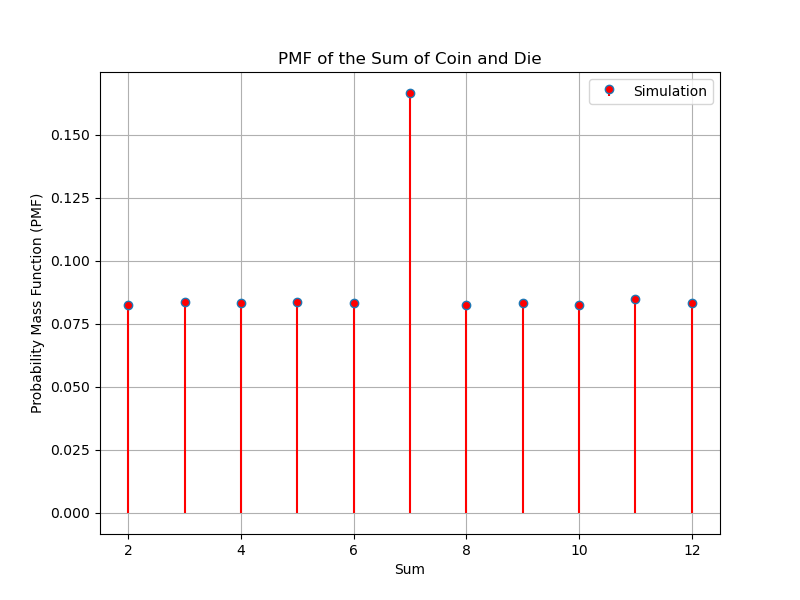
\includegraphics[width=\columnwidth]{figs/pmf.png}
\caption{Probability Mass Funtion}
\label{fig:Plot1} 
\end{figure}

\begin{figure}[h]
\centering
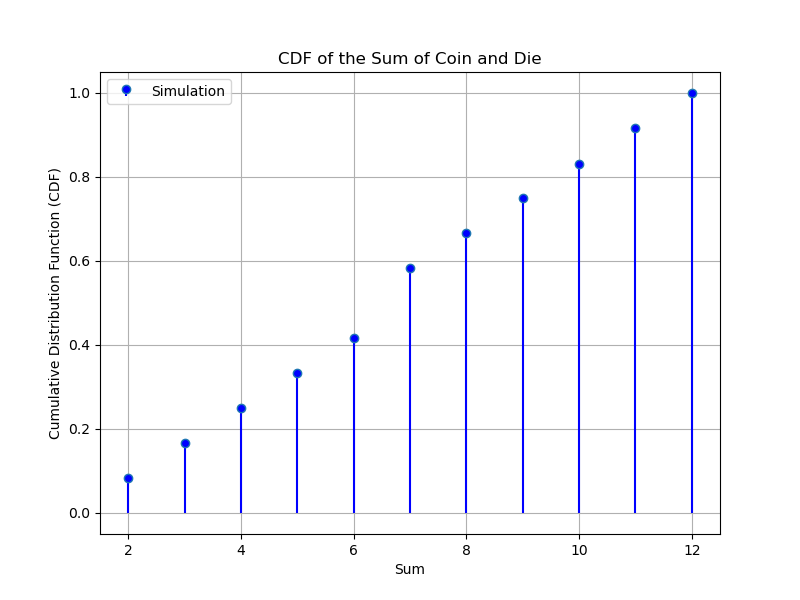
\includegraphics[width=\columnwidth]{figs/cdf.png}
\caption{Cumulative Distribution Function}
\label{fig:Plot1} 
\end{figure}
\end{document}
